\subsubsection{Technologien und Modelle}
\lfoot{Autor: Daniel Melichar}

Wie bereits erwähnt war es von Anfang an klar, dass die komplette Umsetzung der Web-App den Rahmen und benötigten Zeitaufwand um einiges sprengen würde. Es mussten also Modelle und Technologien gefunden werden, die es ermöglichen ein System möglichst modular zu gestalten.

Grundsätzlich besteht jegliche Website (bei Web2.0) aus den folgenden vier Technologien.

\begin{description}
\item[HTML Markup\newline] definiert den Inhalt eines Dokuments und gibt eine Struktur vor mittels dem Einsatz von Sektionen, Überschriften, Paragraphe, Listen, Menüs, und Formulare.

Eine konsequente, saubere, und ersichtliche Struktur ist wichtig da durch den Einsatz von Ankern \textit{(engl.: Hooks)} die weitere Verarbeitung durch CSS und JavaScript passiert. Die Struktur hat auch eine große Wirkung auf die Flexibilität und zuverlässige Bereitstellung der Website.

Durch die Verwendung von Templates, und Standards in einem Projekt, ist es einfacher gewisse Teile einer Web Applikation mehrmals zu verwenden ohne die selbe Arbeit nochmals zu tätigen.

\item[Cascading Style Sheets\newline] oder CSS, ist jener Teil einer Applikation in welcher die visuelle Repräsentation und design Regeln beschrieben werden. Ein gut geschriebenes CSS verwendet das kaskadenförmige Prinzip der Sprache – generelle Regeln werden zuerst inkludiert und danach die überschreibenden für spezifische Instanzen.

Es ist sehr einfach mit CSS inkonsistenten und unnötigen Code zu schreiben, welcher dann so fragil ist, so dass es auf der Webseite immer wieder kleine Unterschiede gibt. Aufgrund dessen sollte CSS immer 
\begin{enumerate}
\item einfach zu Verwalten sein
\item klar ersichtliche Patterns haben
\item das Einfügen von neuen Stilvorgaben ermöglichen
\item nicht verwendete Stilvorgaben weglassen
\item möglichst viele Geräte und Browser Versionen unterstützen
\item Standardwerte setzen
\item Unterscheiden zwischen globalen und spezifischen Styles
\end{enumerate}

Bevor es an das eigentliche Erstellen von Code geht sollte man vorab immer das vorgegebene Design überprüfen, ein technisches Konzept erstellen und hierbei vor allem auf logische Verknüpfungen im Code achten. Das bedeutet konkret, dass man die Styles des Kunden (bzw. deren Corporate Identity) in die Website einplant, die Basis der Typographie der Webseite erstellt, Styles für die komplette Webseite, und danach für einzelne Sektionen, erstellt.

\textbf{Tools und Frameworks\newline}
In manchen Fällen ist die Verwendung von third party libraries sehr hilfreich. Diese sollten aber aus einem guten Grund gewällt werden. Auch hier gibt es wiederum viele Arten von Tools die man verwenden kann. Einige kann man als eigene, bessere Sprachen ansehen welche dann einfach zu CSS umgewandelt werden. Andere reduzieren den bereits vorhanden Code auf das Minimum.

Vorgefertigte UI Komponenten oder CSS Frameworks können ebenfalls sehr hilfreich sein, aber auch hier gilt: nur verwenden, wenn wirklich notwendig. Wiederum gibt es verschiedene Kategorien von Frameworks die für verschiedenstes verwendet werden können: UI Komponenten oder Widget libraries (z.B. Bootstrap, jQuery UI), Grid Systems, Typographie Anpassungen, Normalisierung von Code.


\item[JavaScript\newline]
beschreibt zusätzliche Verhaltensweisen, Features und Funktionalität welche normalerweise nicht von Web Browsern durch den Einsatz von CSS du HTML unterstützt werden. In den letzten Jahren hat JavaScript einen enormen Boom erhalten. Dies ist aufgrund der immer größeren Anzahl an Features, schnelleren Browsern und Server Laufzeitumgebungen wie Node.js. 

Es gibt mittlerweile für beinahe jede Komponente einer Website die man sich vorstellen kann eine JavaScript Library oder Framework. Man sollte dennoch nur dann JavaScript verwenden, wenn keine andere Möglichkeit existiert.  Sollte der Fall eintreten, und es wirklich keine native Funktion durch CSS/HTML geben, muss die JavaScript Komponente auf Performance getestet werden. Auch hier gilt es dann möglichst schnellen, effizienten und performanten, wiederverwendbaren Code zu generieren. 

Für die Auswahl von Third Party Projekten oder Code sollten folgende Punkte bei der Überlegung eingebunden werden:
\begin{enumerate}
\item Technische Requirements 
\item Qualität und Reife
\item Zukünftiger Support
\item Entwickler und Community des Projekts / Code
\item Testung auf verschiedensten Plattformen und Geräten
\end{enumerate}

Viel zu oft vergessen Entwickler von Web-Applikationen das Gesamtkonzept und fokussieren sich nur auf einen geringen Teil - \textit{„Ich füge einfach ein plugin hinzu!“} ist nicht immer eine gute Lösung. Deshalb sollte JavaScript hauptsächlich für die folgenden Komponenten und/oder Eigenschaften verwendet werden
\begin{enumerate}
\item Document Object Model (DOM) Manipulation
\item Ajax Validation
\item Query String Konverter
\item Tests für globale Konditionen (z.B. Bildschirmgröße, Feature Support)
\item UI Controls
\item Datum Selektion
\end{enumerate}
\end{description}

\clearpage

\textbf{Verwendung und Anwendung\newline}
Die folgenden Frameworks und Libaries wurden in Betracht gezogen. Letzendlich haben wir uns dann für \textbf{Anglar 2.0} entschlossen da wir bereits ein wenig Erfahrung mit diesem Framework hatten und somit das negative für uns nicht relevant war. Mit Hilfe des Frameworks war es möglich einen Prototype zu erstellen und die weiteren Bedürfnisse der Web-App zu evaluieren.

\begin{table}[!htb]
\centering
\resizebox{\columnwidth}{!}{%
\begin{tabular}{ll}
\hline
\multicolumn{2}{|c|}{\textbf{Angular 2.0}}                                                                                                                                                                                   \\ \hline
\multicolumn{1}{|c|}{\textbf{Stärken}}                                                                                                                                 & \multicolumn{1}{c|}{\textbf{Schwächen}}             \\ \hline
\multicolumn{1}{|l|}{Performance}                                                                                                                                      & \multicolumn{1}{l|}{Dokumentation ist eher schwach} \\ \hline
\multicolumn{1}{|l|}{Rendering am Server}                                                                                                                              & \multicolumn{1}{l|}{}                               \\ \hline
\multicolumn{1}{|l|}{Native GUI}                                                                                                                                       & \multicolumn{1}{l|}{}                               \\ \hline
\multicolumn{1}{|l|}{\begin{tabular}[c]{@{}l@{}}Herangehensweise eines Frameworks \\ (spezifische Funktionen von Angular \\ können einfach entfernt werden)\end{tabular}} & \multicolumn{1}{l|}{}                               \\ \hline
\multicolumn{1}{|l|}{ES2015 Standard includiert}                                                                                                                       & \multicolumn{1}{l|}{}                               \\ \hline
\multicolumn{1}{|l|}{Große Community}                                                                                                                                  & \multicolumn{1}{l|}{}                               \\ \hline
\multicolumn{1}{|l|}{Einfache testung} & \\ \hline                                                           
\end{tabular}
}
\caption{Angular 2.0 - \url{https://angular.io/}}
\end{table}

\textbf{Angular 2.0} ist ein Framework, welches dabei helfen soll, Client Applikationen in HTML und JavaScript zu entwickeln. Das Framework an sich besteht aus mehreren kooperierenden Libaries. Für die Erstellung einer Angular Applikation muss man so gennante HTML \textit{templates} im Angular-Stil, einige \textit{component} Klassen welche die templates managen, und die Logik hinter der Applikation in so gennanten \textit{services}, schreiben \cite{MELD.CH3-web-app.angular}.

\begin{figure}[!htb]\centering
	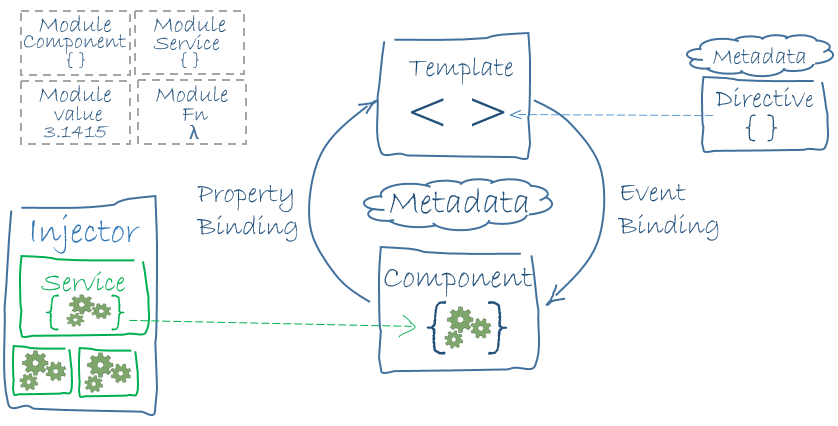
\includegraphics[width=0.8\textwidth]{images/angular}
	\caption{Angular Architektur \cite{MELD.CH3-web-app.angular}}
\end{figure}



\begin{table}[!htb]
\centering
\resizebox{\columnwidth}{!}{%
\begin{tabular}{ll}
\hline
\multicolumn{2}{|c|}{\textbf{Ember 2.0}}                                                                                                                                                                                                                                            \\ \hline
\multicolumn{1}{|c|}{\textbf{Stärken}}                                                                                                                                    & \multicolumn{1}{c|}{\textbf{Schwächen}}                                                                 \\ \hline
\multicolumn{1}{|l|}{Performance}                                                                                                                                         & \multicolumn{1}{l|}{\begin{tabular}[c]{@{}l@{}}Schwirige Anwendung in speziellen\\ Fällen\end{tabular}} \\ \hline
\multicolumn{1}{|l|}{Rendering am Server}                                                                                                                                 & \multicolumn{1}{l|}{Kleinere Community}                                                                 \\ \hline
\multicolumn{1}{|l|}{Native GUI}                                                                                                                                          & \multicolumn{1}{l|}{}                                                                                   \\ \hline
\multicolumn{1}{|l|}{\begin{tabular}[c]{@{}l@{}}Herangehensweise eines Frameworks \\ (spezifische Funktionen von Angular \\ können einfach entfernt werden)\end{tabular}} & \multicolumn{1}{l|}{}                                                                                   \\ \hline
\multicolumn{1}{|l|}{Dokumentation}                                                                                                                                       & \multicolumn{1}{l|}{}                                                                                   \\ \hline
\multicolumn{1}{|l|}{CLI Tools} & \\ \hline                                                                   
\end{tabular}
}
\caption{Ember 2.0 \url{http://emberjs.com/}}
\end{table}

\textbf{Ember.js 2.0} ähnelt sehr stak dem Angulars Architektur Konzept. Der Grund wieso wir uns Ember nicht verwenden basiert auf der simpleren, etwas schöneren API von Angular, und den Fakten, dass Angular keine weiteren Dependencies hat (Ember.js verwendet jQuery und Handlebars) und dass Angular eine viel geringere Filegröße hat \cite{MELD.CH3-web-app.ember}.

\begin{figure}[!htb]\centering
	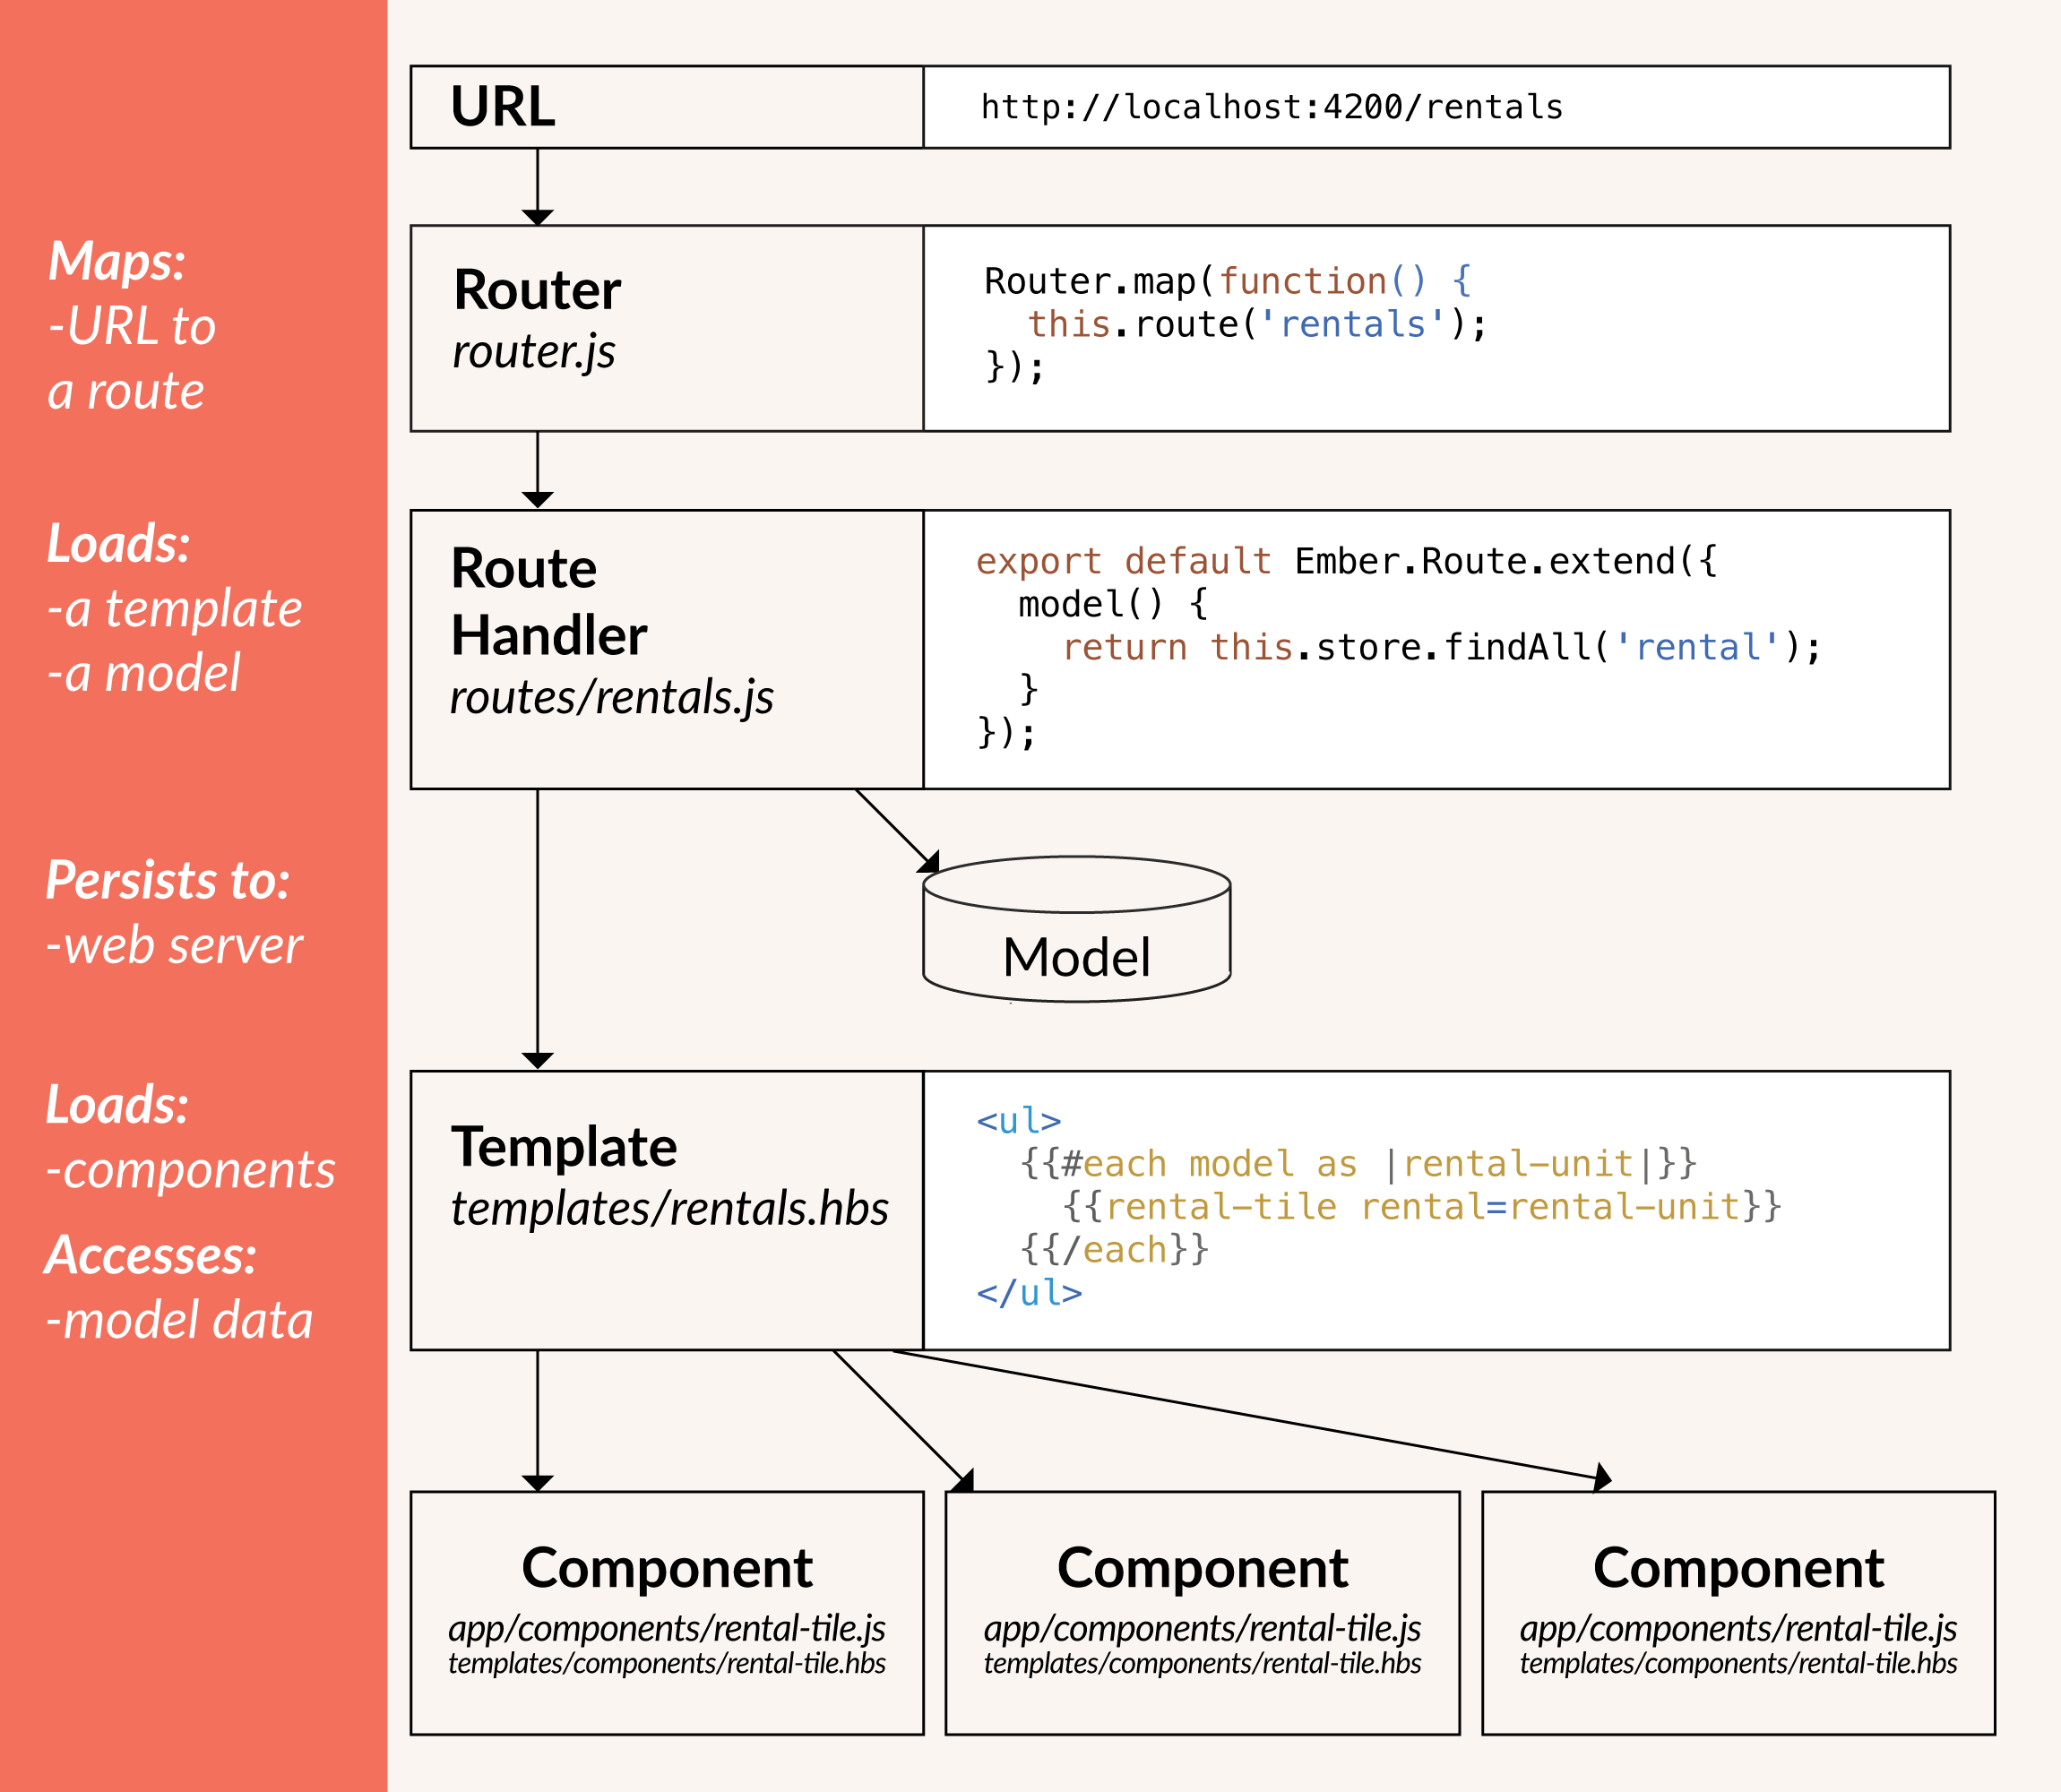
\includegraphics[width=0.6\textwidth]{images/ember}
	\caption{Ember Architektur \cite{MELD.CH3-web-app.ember}}
\end{figure}

\clearpage

\begin{table}[!htb]
\centering
\resizebox{\columnwidth}{!}{%
\begin{tabular}{ll}
\hline
\multicolumn{2}{|c|}{\textbf{React 1.0}}                                                                                                                                                                                                                                                             \\ \hline
\multicolumn{1}{|c|}{\textbf{Stärken}}                                                                                                                                    & \multicolumn{1}{c|}{\textbf{Schwächen}}                                                                                  \\ \hline
\multicolumn{1}{|l|}{Performance}                                                                                                                                         & \multicolumn{1}{l|}{\begin{tabular}[c]{@{}l@{}}Andere Architektur als bei gängigen\\ Frameworks / Libaries\end{tabular}} \\ \hline
\multicolumn{1}{|l|}{Rendering am Server}                                                                                                                                 & \multicolumn{1}{l|}{Unnötig hinzugefügte Features}                                                                       \\ \hline
\multicolumn{1}{|l|}{Native GUI}                                                                                                                                          & \multicolumn{1}{l|}{}                                                                                                    \\ \hline
\multicolumn{1}{|l|}{\begin{tabular}[c]{@{}l@{}}Herangehensweise eines Frameworks \\ (spezifische Funktionen von Angular \\ können einfach entfernt werden)\end{tabular}} & \multicolumn{1}{l|}{}                                                                                                    \\ \hline
\multicolumn{1}{|l|}{Einfach anzuwenden}                                                                                                                                  & \multicolumn{1}{l|}{}                                                                                                    \\ \hline
\multicolumn{1}{|l|}{ES2015 Standard includiert} & \\ \hline                                                                   
\end{tabular}
}
\caption{React 1.0 \url{https://facebook.github.io/react/}}
\end{table}

Das von Facebook entwickelte \textbf{React.js} ist ein eher spezielles Framework, oftmals wird gesagt, dass React.js das \textbf{V} im MVC-Konzept (Model-View-Control) da bietet. Aufgrund dessen ist die Filegröße des Frameworks um einiges kleiner als bei den anderen beiden, bietet aber dennoch viele der Basis Features an \cite{MELD.CH3-web-app.react}. Leider bietet React nicht alles an was für unsere Applikation benötigt wird, daher ging es rasch aus der ängeren Auswall raus.

\begin{figure}[!htb]\centering
	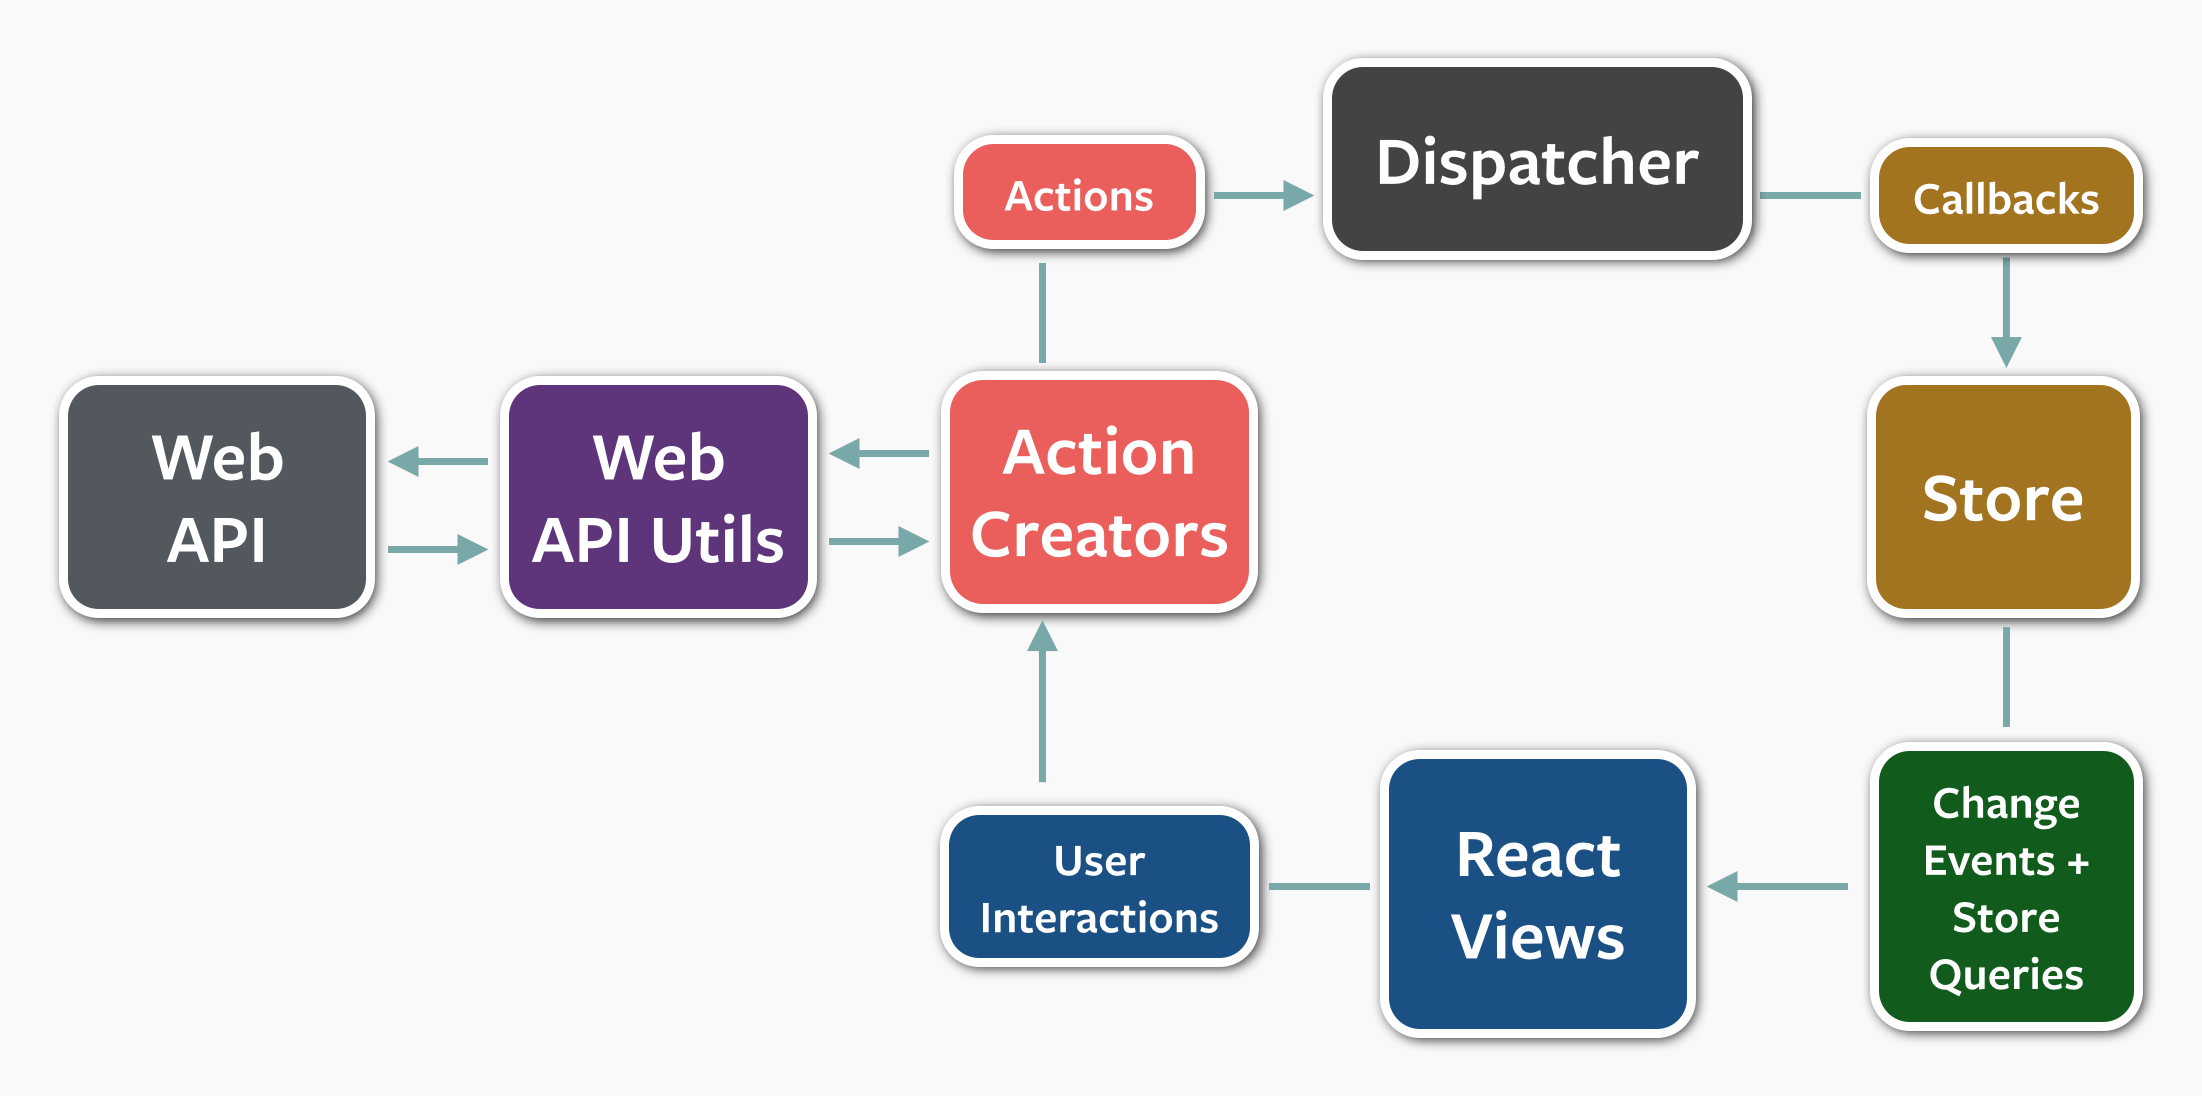
\includegraphics[width=0.8\textwidth]{images/react}
	\caption{React Architektur \cite{MELD.CH3-web-app.react}}
\end{figure}

\clearpage